\documentclass{ltjsarticle}
\usepackage{titlesec}
\usepackage{amsmath, amssymb} % 数学用パッケージ
\usepackage{graphicx} % 図を入れる用
\usepackage{hyperref} % 目次やリンク
\usepackage{physics}


% latexmk -lualatex Maxwell.eq.tex
% 実行コマンド(ターミナルからしか実行できない!?)

\begin{document}
\begin{titlepage}
    \centering
    \vspace*{3cm} % 上からの余白を調整
    {\Huge \bfseries 電磁気学の帰着としての\\特殊相対性理論}\\[1.5cm] % 題名(フォントサイズ大&太字)
    {\Large ~電磁気学が予想する時空~}\\[1cm]
    {\large 北村光瑠}\\[5cm]
    {\large 2025年10月9日}
    \vfill % 下側に空白を自動調整して配置
\end{titlepage}



\section{Abstract}
This study aims to derive the principle of the constancy of the speed of light and the invariance 
under Lorentz transformations from Maxwell's equations, the fundamental equations of electromagnetism. 
We demonstrate that the theoretical structure of electromagnetic fields forms the foundation of special relativity, 
thereby revealing that relativistic physics is a natural consequence inherent in the laws of nature.

\section{Introduction}
本研究では, 電磁気学に内在する理論構造から, 相対性理論が自然界における必然的帰結であることを明らかにする. 
電磁気学は我々の生活に深く関わる学問であり, スマートフォンや照明などの基盤を支えている.
そんな電磁気学から相対性理論を導くことで, 日常生活と物理学との深い結びつきを示すことを目的とする.

\section{Method}
本研究で, 電磁気学におけるMaxwell方程式を用いて, 光速度不変の原理およびLorentz変換の不変性を検証する. 
\subsection{特殊相対性理論}
まず相対性理論(Theory of relativity)は, 1905年にEinsteinによって発表された特殊相対性理論(Special relativity)と, 
その後同じくEinsteinが1915年に発表した一般相対性理論(General Theory of Relativity; GR)の二つに分類できる. 
二つの理論の違いは, 理論の中に重力を含むか含まないかである. 
この二つの中でもまずは重力を含まない特殊相対性理論について解説する. 

特殊相対性理論は重要な二つの原理を土台として成り立っている. 
それは「特殊相対性原理」「光速度不変の原理」である. 
これらの原理により, 特殊相対性理論では
\begin{itemize}
    \item  動くものの時間は遅れる
    \item  動くものの長さは遅れる
    \item 「エネルギー」=「質量」
\end{itemize}
という特徴が表れる. 

\subsubsection{特殊相対性原理}
特殊相対性原理とは「どの慣性系(静止している座標系か等速直線運動している座標系)から見たとしても, 物理法則は不変である」という原理である. 
つまり「静止している」「等速運動している」ということはあくまで相対的でしかないため, 
止まっている観測者から見ても, 一定の速さで動いている観測者から見ても, 物理法則(たとえばNewtonの運動法則やMaxwell方程式)は同じように成り立つ. 
地球上で物体を落下させれば, 通常の物理法則と合致するが, それは等速運動するような座標系でも同じである. 
例として, 電車が一定の速さでまっすぐ走っているとき, その中でボールを投げても, 地上に静止しているときと同じように運動方程式が成り立つ. 

\subsubsection{光速度不変の原理}
光速度は昔, エーテルという媒質を通じて伝わると考えられていた. 
光は波であるため, 音波が空気を通じて伝播されるように何かしらの媒質を通じて伝わると考えられたのである. 
この媒質をエーテルと呼び, エーテルは宇宙に対して静止していると考えられていた. 
ゆえに, 地球がエーテルに対して運動している場合, エーテル風が発生し(図1参照), 光速度は観測者の運動状態によって変化するはずである.
しかし, Michelson-Morleyの実験により, 光速度が観測者の運動状態に依存しないことが示され, エーテルの存在は否定された. 
この実験結果を受けて, Einsteinは光速度を一定とする原理「光速度不変の原理」を提唱した.

\begin{figure}[htbp]
  \centering
  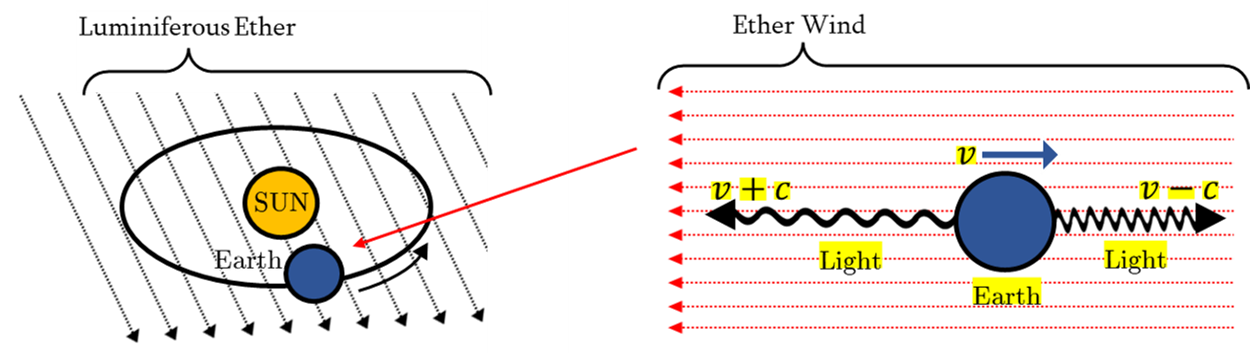
\includegraphics[width=1\textwidth]{img/エーテル.png}
  \caption{エーテル風が存在すると仮定した場合の光速の変化}
\end{figure}

光速度不変の原理とは「どの慣性系から見ても光の速さは変わらない」(観測者の運動状態に依存しない)というものだ. 
例えば, 静止しているAと, $x$方向に$v~\mathbf{m/s}$で移動しているBから, $x$方向に$c~\mathbf{m/s}$で動く光$c$を考える. 
もちろんAから見た$c$の速度は$c~\mathbf{m/s}$であるが, Bから$c$の速度を見たとしても$v + c ~\mathbf{m/s}$とはならず, $c~\mathbf{m/s}$と見える. 
こうした光速度が一定に保たれてしまうような不思議な原理をまずは認めなければならない. この原理は実験により証明されている. 
この原理を成り立たせるために特殊相対性理論ではLorentz変換を利用し, 理論体系を構築している. 
Lorentz変換を知るために, まずは座標変換について学ばなければならない. 



\subsection{Maxwell方程式と光速度}
真空中のMaxwell方程式の微分形から波動方程式を導出し, 光速 $c$ を得る. 
これにより, 光が電磁波の一種であることを理解する. 
ただし,この段階で得られるのはあくまで「電磁波の伝播速度が一定である」という結果であり,
「すべての慣性系で光速度が不変である」という原理そのものの説明には至らない.
この点については, 次節でLorentz変換の導入を通じて理論的に明らかにする.

\subsubsection{波動方程式の解説}
まず, 導出のための準備として波動方程式について説明する. 
波動方程式とは, 波の伝播を記述する偏微分方程式で, 簡単な力学の知識で導出することができる.
最初に, テイラー展開による計算の簡略化を説明する. 

\subsection*{テイラー展開}
テイラー展開は, 無限回微分可能な一般の関数 $f(x)$ について,以下の等式が成立する. 
この等式をテイラー展開といい,  特に, 原点でのテイラー展開をマクローリン展開という. 
\begin{equation}
  f(x) = \sum_{k=0}^n \frac{f^{(k)}(a)}{k!} (x - a)^k
\end{equation}
となる. これを利用して, 三角関数のテイラー展開を考えると
\begin{equation}
  \sin x = x - \frac{x^3}{3!} + \frac{x^5}{5!} - \cdots 
\end{equation}
\begin{equation}
  \cos x = 1 - \frac{x^2}{2!} + \frac{x^4}{4!} - \cdots
\end{equation}
\begin{equation}
  \tan x = x + \frac{x^3}{3} + \frac{2x^5}{15} + \cdots
\end{equation}
$x \ll 0$のとき高次項(曲率)は無視できるので, 一次テイラー展開(一次近似)は
\begin{equation}
  f(x) \simeq f(a) + f'(a)(x - a)
\end{equation}
角度が微小な場合の一次テイラー展開は
\begin{equation}
  \tan x \simeq x, \quad \sin x \simeq x, \quad \cos x \simeq 1
\end{equation}
よって
\begin{equation}
  \tan x \simeq \sin x
\end{equation}
\begin{equation}
  \cos x \simeq 1
\end{equation}
という関係が得られる. これが, 高校で学んだ「微小角の近似」が許される理由である.

さらに, テイラー展開を利用して, 平方根についても近似することができる. 
\begin{equation}
  f(x) = \sqrt{1 + x }
\end{equation}
を$x$が微小な場合について一次テイラー展開すると
\begin{equation}
  f(x) \simeq f(0) + f'(0)(x - 0)
\end{equation}
\begin{equation}
  f'(x) = \frac{d \sqrt{1 + x}}{dx} = (1 + x)^{\frac{1}{2}} = \frac{1}{2 \sqrt{1 + x}}
\end{equation}
\begin{equation}
  f(0) \simeq \frac{1}{2}
\end{equation}
よって, 平方根の近似$f(x)$は以下のようになる. 
\begin{equation}
  f(x) = \sqrt{1 + x } \simeq 1 + \frac{1}{2} x \quad (x \ll 0)
\end{equation}

\subsection*{テイラー展開と波動方程式の導出}
では実際に波動方程式を導出していこう. 
初めに, 導出する波動方程式を以下に表す. 
\begin{equation}
  \frac{\partial^2 u}{\partial t^2}=v^2 \frac{\partial^2 u}{\partial x^2}
\end{equation}

まず, ピンと張った弦を弾いた時の弦の振動について考える. 
その弦全体と微小要素の図を図3に示した. 
\begin{figure}[htbp]
  \centering
  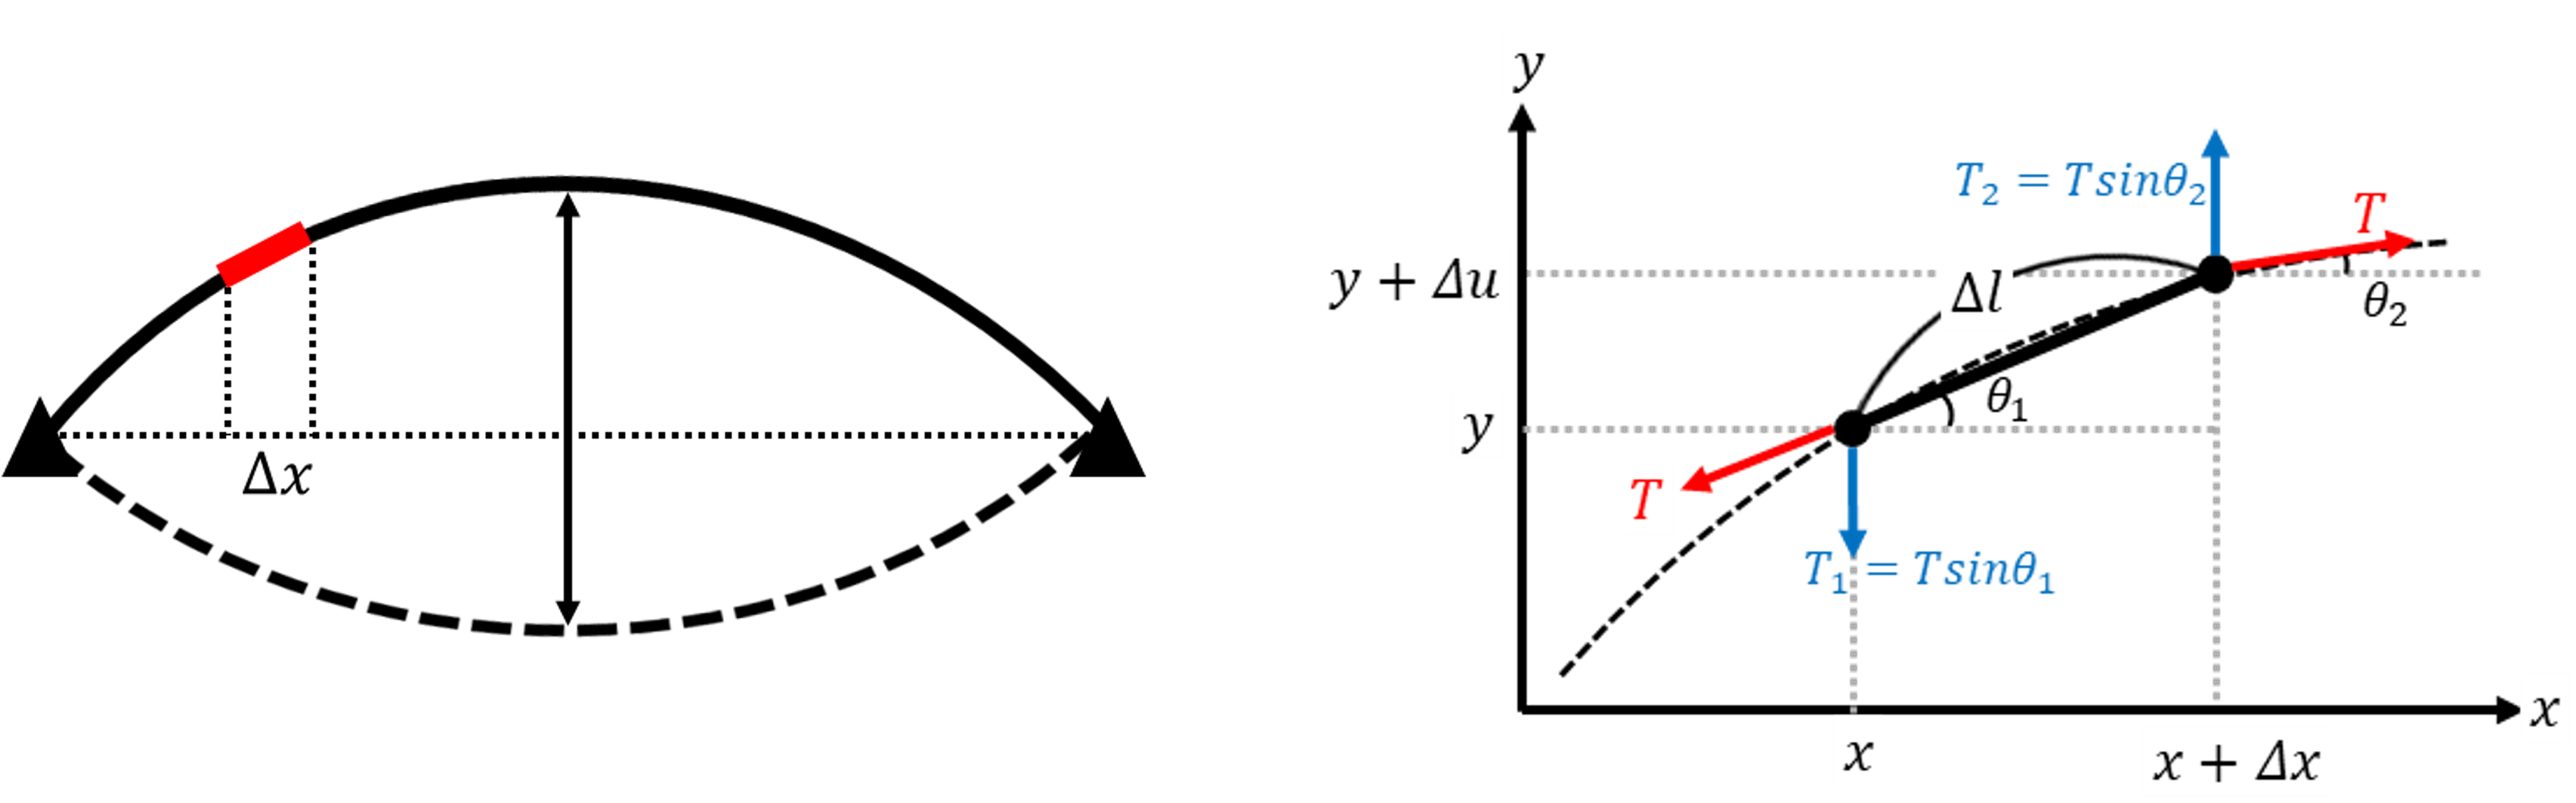
\includegraphics[width=1\textwidth]{img/弦の振動.png}
  \caption{弦の振動を模式的に表した図}
\end{figure}
この微小要素の両端には張力$T[N]$が働き, 一定であるのでどちらも同じ大きさである. 
点$A$では$\theta_1$方向に, 点$B$では$\theta_2$方向に張力が働く. 
$\Delta x$を微小と考えることでAB間を直線とみなしているが, その外側ではその限りではないので
$\theta_1 \neq \theta_2$となる.

弦は一般に張力によって上下に振動するが, 張力が上下ではなく斜めに加わっているため, 左右に振動する可能性もある. 
しかし, 現実世界では横方向に振動する弦は存在しない. この現象は, Tの力の分解によって得ることができる. 
(15)式より

\begin{equation}
  T \cos θ_1 = T \cos θ_2
\end{equation}

となる. つまり, $x$方向の張力は釣り合っていることがわかる. 
これが, 横方向に弦が振動しない理由である. 

では鉛直方向の力の分解を考える. 点AでのTの$y$成分を$T_1$, 点BでのTの$y$成分を$T_2$とすると, (14)式より
\begin{equation}
  T_1 = T \sin θ_1 \simeq T \tan θ_1 = \lim_{\Delta x \to 0} T \frac{\Delta u}{\Delta x} = T \frac{\partial u(x,t)}{\partial x}
\end{equation}
微小角近似と(9)式の一次テイラー展開を利用して, 
\begin{equation}
  T_2 = T \sin θ_2 \simeq T \tan θ_2 = T \frac{\partial u(x + \Delta x ,t)}{\partial x}
\end{equation}
\begin{equation}
  u(x + \Delta x ,t) \simeq u(x, t) + \frac{\partial u(x ,t)}{\partial x} \Delta x
\end{equation}
\begin{equation}
  T_2 \simeq T \reft{  \frac{\partial u(x ,t)}{\partial x} + \frac{\partial^2 u(x ,t)}{\partial x^2} \Delta x  \right}
\end{equation}
ゆえに鉛直方向に働く力$F$は
\begin{equation}
  F = T_2 - T_1 = T \frac{\partial^2 u(x ,t)}{\partial x^2} \Delta x
\end{equation}

これで力の大きさを得ることができたが, 力の向きは正負どちらの方向に働くのだろうか?
$T_1$が$T_2$より下にあるので, $θ_1 \textgreater \theta _2$となる. 
ゆえに, $\sin θ_1  \textgreater \sin \theta _2$より$T_1  \textgreater T_2$という関係が得られる. 
この関係より, 負の方向に力$F$が働くことがわかる. 

さらに, 弦の曲率の関係から力の働く方向を導くことができる. 
曲率は関数を二階微分することで得られ, その値が正であると上に凸, 負であると下に凸であるとわかる. 
(27)式より, $F$は弦の関数$u(x, t)$を$x$について偏微分し, $\Delta x$と$T$をかけたものである. 
つまり, 弦の曲率に$\Delta x$と$\Delta x$と$T$をかけたものだと考えることができる. 
よって図3より, 弦が上に凸の形状をしているため, 弦の曲率は負であると考えることができ, $F$は負であるとわかる. 
\begin{figure}[htbp]
  \centering
  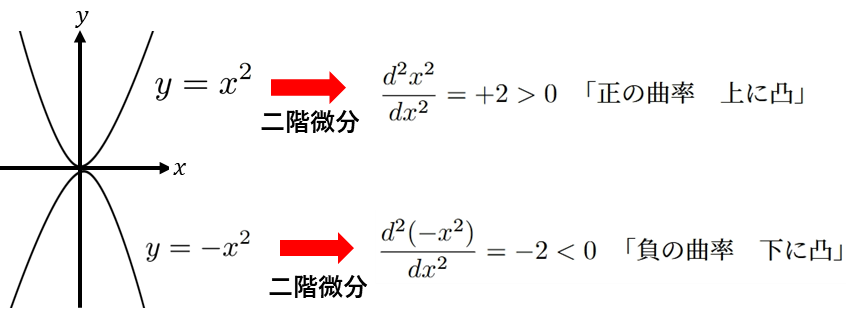
\includegraphics[width=0.8\textwidth]{img/曲率.png}
  \caption{二次関数の曲率}
\end{figure}
では, この弦に働く力$F$について運動方程式を立てよう. 
微小要素の質量を$m$とすると
\begin{equation}
  F = m \frac{\partial^2 u(x ,t)}{\partial t^2}
\end{equation}
微小要素の単位長さ当たりの質量を表す線密度を$\rho$とすると$m$は次のように表せる. 
\begin{equation}
  m = \rho \Delta l
\end{equation}
\begin{equation}
  \Delta l = \sqrt{(\Delta x)^2 + (\Delta u)^2} = 
  \sqrt{(\Delta x)^2 \{ 1 + \left(\frac{\Delta u}{\Delta x}\right)^2 \} } = \Delta x \sqrt{1 + \left(\frac{\Delta u}{\Delta x}\right)^2}
\end{equation}
これを代入し, 極限をとって
\begin{equation}
  m = \rho \Delta x \sqrt{1 + \left(\frac{\Delta u}{\Delta x}\right)^2} =
  \rho \Delta x \sqrt{1 + \left( \frac{\Delta u}{\Delta x} \right)^2}
\end{equation}
平方根の近似より
\begin{equation}
  m = \rho \Delta x \left( 1 + \frac{1}{2} \frac{\partial^2 u(x ,t)}{\partial x^2} \right)
\end{equation}
$\theta_1 \ll 0$より, $u(x,t)$の$x$方向の曲率はほぼゼロであるので
\begin{equation}
  m = \rho \Delta x 
\end{equation}
\begin{equation}
  F = \rho \Delta x \frac{\partial^2 u(x ,t)}{\partial t^2}
\end{equation}
(20)式を代入すると
\begin{equation}
  \frac{\partial^2 u(x ,t)}{\partial x^2} \Delta x= \frac{\rho}{T} \frac{\partial^2 u(x ,t)}{\partial t^2}
\end{equation}
$T[N]=[kg \cdot m/s^2], \rho [kg/m]$より
\begin{equation}
  \frac{\rho}{T}=\frac{[kg/m]}{[kg \cdot m/s^2]}=\frac{1}{[m^2/s^2]}
\end{equation}
よって, 一次元の波動方程式は
\begin{equation}
  \frac{\partial^2 u}{\partial x^2} \Delta x= \frac{1}{v^2} \frac{\partial^2 u}{\partial t^2}
\end{equation}

ラプラシアンを
$
\nabla^2 = \left( \frac{\partial^2}{\partial x^2}, \frac{\partial^2}{\partial y^2}, \frac{\partial^2}{\partial z^2} \right)
$, 弦の関数を
$
, \psi (\mathbf{r}, t), \mathbf{r} = (x, y, z)
$
とすると3次元の場合の波動方程式は以下のように記述できる. 
\begin{equation}
  \nabla^2 \psi= \frac{1}{v^2} \frac{\partial^2 \psi}{\partial t^2}
\end{equation}




% \textgreater → >
% \textless    → <
% \quad 空白

\subsubsection{電磁波の導出}
真空中における微分形のMaxwell方程式は, 以下のように与えられる. 
\begin{equation}
  \begin{cases}
    \nabla \cdot \mathbf{E} = 0  &\text{①} \\
    \nabla \cdot \mathbf{B} = 0  &\text{②} \\
    \nabla \times \mathbf{E} = -\,\frac{\partial \mathbf{B}}{\partial t}  &\text{③} \\
    \nabla \times \mathbf{B} = \mu_0 \varepsilon_0 \frac{\partial \mathbf{E}}{\partial t} &\text{④}
  \end{cases}
\end{equation}
④式を時間微分し, ②式より磁場の時間微分を電場のローテーションに書き換えられるので, 
\begin{equation}
  \nabla  \times \frac{\partial \mathbf{B}}{\partial t} = \mu_0 \varepsilon_0 \frac{\partial^2 \mathbf{E}}{\partial t^2}
\end{equation}
\begin{equation}
  \nabla  \times ( -\nabla \times \mathbf{E} ) = \mu_0 \varepsilon_0 \frac{\partial^2 \mathbf{E}}{\partial t^2}
\end{equation}
となる. ベクトル恒等式
\begin{equation}
  \nabla \times (\nabla \times \mathbf{A}) = \nabla(\nabla \cdot \mathbf{A}) - \nabla^2 \mathbf{A}
\end{equation}
と①式を用いると,
\begin{equation}
  \nabla \times (-\nabla \times \mathbf{E}) = -\nabla \times (\nabla \times \mathbf{E}) = -(\nabla(\nabla \cdot \mathbf{E}) - \nabla^2 \mathbf{E})
\end{equation}
\begin{equation}
  -(\nabla(0) - \nabla^2 \mathbf{E}) = \nabla^2 \mathbf{E}
\end{equation}
\begin{equation}
  \nabla^2 \mathbf{E} = \mu_0 \varepsilon_0 \frac{\partial^2 \mathbf{E}}{\partial t^2}
\end{equation}
全く同じ手順で磁場の波動方程式を導出すると, 以下のように磁場の波動方程式を導出できる. 
\begin{equation}
  \nabla^2 \mathbf{B} = \mu_0 \varepsilon_0 \frac{\partial^2 \mathbf{B}}{\partial t^2}
\end{equation}
よって, 波動方程式
\begin{equation}
  \nabla^2 \psi = \frac{1}{v^2} \frac{\partial^2 \psi}{\partial t^2}
\end{equation}

より, $v$ は波の速度なので(1)式および(2)式より, 電磁波の速度 $v_e$ は

\begin{equation}
  \mu_0 \varepsilon_0 = \frac{1}{ (\frac{1}{\mu_0 \varepsilon_0}) } = \frac{1}{ \sqrt{(\frac{1}{\mu_0 \varepsilon_0})^2} }
\end{equation}

\begin{equation}
  v_e = \frac{1}{\sqrt{\mu_0 \varepsilon_0}}
\end{equation}

SI単位系において, 真空の透磁率 $\mu_0 = 1.25663706 \times 10^{-6} \mathrm{H/m}$, 真空の誘電率 $\varepsilon_0 \simeq 8.85418781 \times 10^{-12} \mathrm{F/m}$ であるので

\begin{equation}
  v_e = \frac{1}{\sqrt{1.25663706 \times 10^{-6} \times 8.85418781 \times 10^{-12}}} \simeq 2.99792458 \times 10^8 \mathrm{m/s}
\end{equation}

したがって, $v_e$は光速度 $c \simeq 2.99792458 \times 10^8 \mathrm{m/s}$ と一致する. すなわち, Maxwell方程式から光速度 $c = 1/\sqrt{\varepsilon_0 \mu_0}$ を導出できた. こ
れは光速度が媒質に依存しないことを示しており, エーテルの存在を否定できる.

\subsection{Lorentz変換と不変性}
Galilei変換では光速度不変の原理が成り立たない. 
これを解決するためにLorentz変換を導入し, Maxwell方程式がLorentz変換の下で不変であることを確認する. 
これにより, 電磁気学が相対論的枠組みを内包していることを示す. 

\subsubsection{Lorentz変換の導出}
Maxwell方程式がLorentz不変であることを示すための準備として, まずはLorentz変換を導出する. 

そもそも座標変換とは何か. 
一番直感的で身近なのは古典力学における大前提「Galilei変換」である. 
ある座標系 \(S'\) が速度 \(\mathbf{v} = (v_x, v_y, v_z)\) で移動しているとき, 
位置と時間のGalilei変換は

\begin{equation}
\begin{cases}
x' = x - v_x t \\
y' = y - v_y t \\
z' = z - v_z t \\
t' = t
\end{cases}
\end{equation}

ここで
\((x, y, z, t)\) : 静止系 \(S\) の座標
\((x', y', z', t')\) : 移動系 \(S'\) の座標  
時間は絶対 (\(t' = t\))  (どの座標系のどのような位置でも時間は同じであるということ)

これを具体例で考えてみる. 
ボールを$x$軸方向に$5\mathbb{m/s}$で投げる. 
3秒後に, 静止しているAからボールを観測した場合, ボールの座標は

\begin{equation}
0 - (5 \times 3)= -15\mathbf{m}
\end{equation}

となる. 

\begin{figure}[htbp]
  \centering
  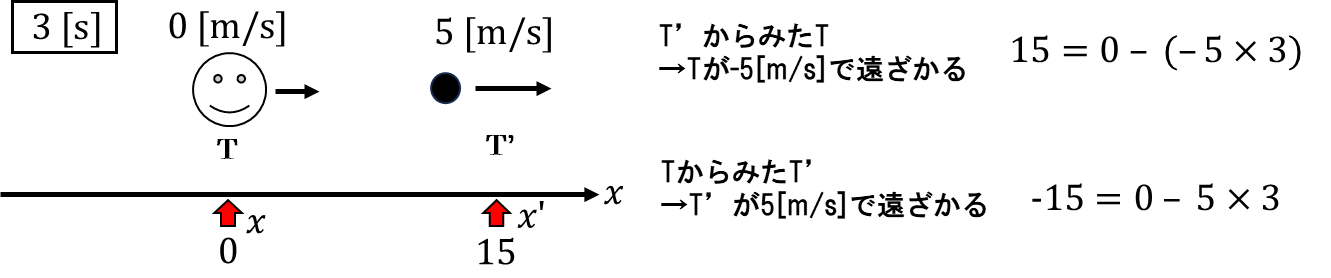
\includegraphics[width=1\textwidth]{img/Galilei変換.png}
  \caption{Galilei変換の図}
\end{figure}

この結果を, 先ほど示したGalilean変換式を用いて表現してみる. 
$x$軸方向に速度$v = 5\mathbf{m/s}$で動くボールを座標系$T'(x', y', z', t')$とし, 静止しているAを座標系$T(x, y, z, t)$とすると位置と時間のGalilei変換は

\begin{equation}
\begin{cases}
x' = x - vt = x - 5 t \\
y' = y \\
z' = z \\
t' = t
\end{cases}
\end{equation}
速度は位置を時間で微分すればよいので(どのくらいの時間でどれだけ変化したか)
\begin{equation}
\begin{aligned}
v_x &= \frac{dx}{dt} = \frac{d}{dt}(x' + v t) = \frac{dx'}{dt} + \frac{d(vt)}{dt} = v'_x + v = 5 + 0 = 5\mathbf{m/s}
\end{aligned}
\end{equation}
ここで, $v_x$ 観測者Aから見たボールの速度, $v'_x$はボールの速度, $v$ は観測者Aの速度である. 

これは, 先ほどの加算式と完全に一致する. 
このように異なる座標系(Aから見たボールの見え方と, ボールから見たAの見えかたは違う→座標系が違う )間で, 
相対速度を計算し, 別の座標系での表現に変換することを座標変換という. 
特に, この「$t' = t$ どの座標系のどの位置でも時間は同じ(絶対的である)」というような座標変換がGalilei変換である. 

しかし, この座標変換では光速度不変の原理を成り立たせることはできないのである. 光速を$c$とおき, 
$x$軸方向に速度$0.7c\mathbf{m/s}$で動く電車を座標系$T'$とし, 車内にいるBが$x$軸方向に$0.5c\mathbf{m/s}$でボールを投げる. 
静止しているAを座標系$T$とすると$T$と$T'$における, 位置と時間のGalilei変換は
\[
0.5c + 0.7c = 1.2c
\]
よって光速は常に$c$であるという光速度不変の原理が成り立たなくなってしまう. 
そこで今度は, 光速度$c$が常に一定になるような変換を考えてみる. 

普通に, $x$ 軸方向に速度 $v$ で運動する慣性系 $K'$ と,静止している慣性系 $K$ の間での座標変換を導出しよう. 
導出するときのポイントとして
\begin{itemize}
    \item 空間が等方的
    \item 各軸が回転せず各軸が垂直に交わる
    \item $t = 0$の時に原点が重なる
\end{itemize}
このことを仮定する. 

手始めに, 進行方向に対して垂直な成分$y', z'$について考える. 
$y'$軸は$xz$平面に対して垂直で, $K'$系が$x$方向にしか進んでいないことより$y'$は$t$に依存していないことがわかる. 
ゆえに, $y'$は相対速度$v$に依存した係数$a$に比例することがわかる. 
\begin{equation}
  y'=ay \quad(aはvに依存) 
\end{equation}
\begin{equation}
  y = ay' \quad 逆方向の変換も同様
\end{equation}
(5)式に(4)式を代入し, 軸が反転しないことより
\begin{equation}
  y' = a^{2} y' \quad a^2=1 \quad a=1
\end{equation}
\begin{equation}
  y' = y
\end{equation}
zも同様にして
\begin{equation}
  z' = z
\end{equation}

次に$x$について考えよう. 
$x$軸方向に速度$v$で動いていることより, 各係数を交えて$x'$の座標変換を書くと
\begin{equation}
  x' = b_1(x - vt) + b_2y + b_3z
\end{equation}
仮定より$t = 0$の時$x=x'=0$となるので$b_2 = b_3 = 0$, $b_1 = b$とすると
\begin{equation}
  x' = b(x - vt)
\end{equation}
最後に時間についてこのような変換をすると
\begin{equation}
  t’=d_1 x+d_2 y+d_3 z+d_4 t
\end{equation}
全体の変換をまとめると次のようになる. 
\begin{equation}
\begin{cases}
x' = x' = b(x - vt) \\
y' = y \\
z' = z \\
t' = t’ = d_1 x + d_2 y + d_3 z + d_4 t
\end{cases}
\end{equation}

これで準備が整ったので, 実際に特殊相対論的な議論をしていく. 
まず各座標系$K, K'$の原点から, 光が放たれる場合を考えよう. 
空間が等方的なので, 同心円状に光が広がっていくと, 円の方程式で光を表すことができる
光速度を$c$とすると
\begin{equation}
  静止系K \quad x^2 + y^2 + z^2 = (ct)^2 
\end{equation}
\begin{equation}
  慣性系K' \quad x'^2 + y'^2 + z'^2 = (ct')^2
\end{equation}

光速度不変の原理より(15)式の慣性系$K'$の方程式にLorentz変換した量を代入すると, (14)式の静止系$K$の方程式と一致するはずである.
この等式を解いて(13)式の各係数を決定していくことによってLorentz変換を完成させていこうと思う. 
(15)式に(13)式を代入し、右辺について展開する
\begin{equation}
  b^2(x - vt)^2 + y^2 + z^2 = c^2(d_1 x + d_2 y + d_3 z + d_4 t)^2
\end{equation}
この式を, 左辺, 右辺について展開すると
\begin{equation}
  b^2(x - vt)^2 + y^2 + z^2 =
  b^2 x^2 -2b^2 vtx + b^2 v^2 t^2 + y^2 +z^2
\end{equation}
\begin{align}
c^2(d_1 x + d_2 y + d_3 z + d_4 t)^2
&= c^2 d_1^2 x^2 + c^2 d_2^2 y^2 + c^2 d_3^2 z^2 + c^2 d_4^2 t^2 \notag\\
&\quad + 2c^2 d_1 d_2 xy + 2c^2 d_1 d_3 xz + 2c^2 d_1 d_4 xt \notag\\
&\quad + 2c^2 d_2 d_3 yz + 2c^2 d_2 d_4 yt + 2c^2 d_3 d_4 zt
\end{align}

この時右辺に, 目指している(14)式に存在しない混合項$xz, yz, yt, zt$が存在する. 
これを消去するために, $d_2 = d_3 = 0$とする. 
このとき, 展開の過程で $c^2 d_2^2 y^2$及び$c^2 d_3^2 z^2$の項に含まれる $y^2, z^2$は一見消失するように見えるが, 
左辺にはそれぞれ独立した$y^2, z^2$の項が既に存在するため, 全体としてそれらの寄与は保持される. 

この消去の物理的解釈として, $d_2 = d_3 = 0$とすると$0 \cdot y^2, 0 \cdot z^2$となる. 
これは$K'$系が$x$方向にしか動いていないため, $y, z$方向が運動に関与していないと考えることができる. 

これらを踏まえ, (18)式をもう一度展開すると
\begin{equation}
  c^2(d_1 x + d_4 t)^2 = c^2 d_1^2 x^2 + c^2 2 d_1d_4 xt + c^2 d_4^2 t^2
\end{equation}
\begin{equation}
  b^2 x^2 -2b^2 vtx + b^2 v^2 t^2 + y^2 +z^2 = c^2 d_1^2 x^2 + c^2 2 d_1d_4 xt + c^2 d_4^2 t^2
\end{equation}
ゆえに, 未知係数が$b, d_1, d_4$となる. (14)式のように整理すると
\begin{equation}
  (b^2 - c^2 d_1^2)x^2 + y^2+ z^2 = (c^2 d_4^2 - b^2 v^2)t^2 +2(c^2 d_1 d_4 + b^2 v)xt
\end{equation}
よって以下のような三元二次連立方程式が得られる. 
\begin{equation}
\begin{cases}
b^2 - c^2 d_1^2 = 1 \quad ①\\
c^2 d_4^2 - b^2 v^2 = c^2 \quad ②\\
c^2 d_1 d_4 + b^2 v = 0 \quad ③
\end{cases}
\end{equation}
まずは$d_4$について解く. ①より得られる(23)式を②, ③に代入すると(24), (25)式が得られる. 
\begin{equation}
  b^2 = 1 + c^2 d_1^2
\end{equation}
\begin{equation}
  c^2 d_4^2 =  c^2 d_1^2 v^2 + v^2 + c^2
\end{equation}
\begin{equation}
  c^2 d_1 d_4 + v + c^2 d_1^2= 0 
\end{equation}
(25)式を移項して二乗すると
\begin{equation}
  c^4 d_1^2 d_4^2 +  = (v + c^2 d_1^2v)^2
\end{equation}
(24)式を$c^2$で割り, (26)式に代入して整理すると
\begin{equation}
  c^4 d_1^2 (d_1^2 v^2 + \frac{v^2}{c^2} + 1) +  = (v + c^2 d_1^2v)^2
\end{equation}
\begin{equation}
  c^4 d_1^4 v^2 + c^2 d_1^2 v^2 + c^4d_1^2 = c^4 d_1^2 v^2 + 2c^2 d_1^2 v^2 + v^2
\end{equation}
\begin{equation}
  c^4 d_1^2 v^2 - c^2 d_1^2 v^2 = v^2
\end{equation}
\begin{equation}
  d_1^2 = \frac{v^2}{c^2} \frac{1}{c^2 - v^2}
\end{equation}
(30)式を(24)式に代入すると
\begin{equation}
  c^2 d_4^2 =  c^2 (\frac{v^2}{c^2} \frac{1}{c^2 - v^2}) v^2 + v^2 + c^2
\end{equation}
\begin{equation}
  d_4^2 =  \frac{v^4}{c^2(c^2 - v^2)} + \frac{v^2}{c^2} + 1 = \frac{c^2}{c^2(c^2 - v^2)} = \frac{1}{1 - \frac{v^2}{c^2}}
\end{equation}
となる. 
(24)式に(32)式を代入して整理すると以下が得られる. 
\begin{equation}
  d_1^2=\frac{v^2}{c^2}\frac{1}{c^2-v^2}
\end{equation}
次に, 式(33)を式(23)に代入すると, 式(27)が得られる. 
\begin{equation}
  b^2=\frac{1}{1-\frac{v^2}{c^2}}
\end{equation}

$v = 0$ の極限を考える. 
このとき各座標系が重なっているので,  $x’= b (x - 0 \cdot t)$より$b \textgreater 0$であるとわかる. ゆえに
\begin{equation}
  b=\frac{1}{\sqrt{1-\frac{v^2}{c^2}}}
\end{equation}
同じように座標系が重なっていると$t = t', x = x'$のように, Lorentz変換は当然「単なる恒等変換」になるはずである. 
$t' = d_1 x +d_4 t$がこの条件を満たすには $d_1 = 0, d_4 = 1$である必要がある. 
これより,  $d_4 \textgreater 0$が得られる. よって
\begin{equation}
  d_4 = \frac{1}{\sqrt{1 - \frac{v^2}{c^2}}}
\end{equation}
最後に, (22)式の③に(35), (36)式を代入すると$d_1$が求まる. 
\begin{equation}
  d_1=-\frac{\frac{v}{c^2}}{\sqrt{1-\frac{v^2}{c^2}}} 
\end{equation}

3つの未知係数$b, d_1, d_4$が求まったので, 実際に(13)式に代入し, Lorentz変換を導出しよう. 
$\omega = ct , \omega' = ct' $とすると
\begin{equation}
  t' = \frac{t - \frac{vx}{c^2}}{\sqrt{1 - \frac{v^2}{c^2}}}
\end{equation}
\begin{equation}
  \omega' = c \frac{t - \frac{vx}{c^2}}{\sqrt{1 - \frac{v^2}{c^2}}} = \frac{\omega - \frac{vx}{c}}{\sqrt{1 - \frac{v^2}{c^2}}}
\end{equation}
\begin{equation}
  x' = \frac{x - vt}{\sqrt{1 - \frac{v^2}{c^2}}} = \frac{x - \frac{v}{c}\omega}{\sqrt{1 - \frac{v^2}{c^2}}}
\end{equation}

また, 式の中に出てきている形を次の文字で置き換える. 
$\beta$は光速に対する相対速度$v$を表し, $\gamma$はローレンツ因子と呼ばれる. 
\begin{equation}
  \beta = \frac{v}{c}, \quad \gamma = \frac{1}{\sqrt{1 - \frac{v^2}{c^2}}}
\end{equation}
(39)式より
\begin{equation}
  \omega' = \gamma (\omega - \beta x)
\end{equation}
よって$x', t'$についてのLorentz変換は
\begin{equation}
  x' = \gamma (x - \beta \omega)
\end{equation}
\begin{equation}
  t' = \gamma \left( t - \dfrac{\beta x}{c}  \right)
\end{equation}

% 
% \left(  \right)
% \textgreater → >
% \textless    → <
% \quad 空白
$x', y', z', t'$についてのLorentz変換をまとめると, 以下のようになる. 
\begin{equation}
\begin{cases}
x' = \gamma (x - \beta \omega) \\
y' = y \\
z' = z \\
t' = \gamma \left( t - \dfrac{\beta x}{c} x \right)
\end{cases}
\end{equation}

では, このLorentz変換を用いて実際に光速に近い系の運動を考えてみる. 
静止系$S, (x, t)$と, $x$軸方向に速度$v = 0.6c$で動く慣性系$S'(x', t')$があり, $(x, t)= (3, 2)$でイベントが起きたとしよう. 
このとき, $\gamma$は
\begin{equation}
  \gamma = \frac{1}{\sqrt{1 - \frac{v^2}{c^2}}} = \frac{1}{\sqrt{1 - 0.36}} = 1.25
\end{equation}

Lorentz変換式は次のように与えられる
\begin{equation}
\begin{cases}
x' = \gamma (x - vt) \\
t' = \gamma \left( t - \dfrac{v x}{c^2} \right)
\end{cases}
\end{equation}
よって$c=1$として各値を代入すると
\begin{equation}
\begin{aligned}
x' &= 1.25 (3 - 0.6 \times 2) = 1.25 \times 1.8 = 2.25 \\
t' &= 1.25 (2 - 0.6 \times 3) = 1.25 \times 0.2 = 0.25
\end{aligned}
\end{equation}

つまり, 静止系$S$で$(x, t)= (3, 2)$のときに起きたイベントは, $0.6c$で動く慣性系$S'$から観測すれば
$(x', t')= (2.25, 0.25)$と見える. 
空間である$x$軸は光速に近い速度で動くことで$0.75$だけ縮み, 時間$t$は$1.75$と時間の経過が異なる. 
これは特殊相対性理論の基本的な効果を示している. 
特に, $x$の変換により静止系での長さが短く見えるのがローレンツ収縮であり, $t$の変換によって異なる系で同時刻の出来事がずれることを同時の相対性という. 












\subsection{Minkowski時空の構成}

\section{Results}
Maxwell方程式から光速 $c = 1/\sqrt{\varepsilon_0 \mu_0}$ を導出し、光速度不変の原理を理論的に証明した。
また、Lorentz変換を施してもMaxwell方程式の形が変わらないことを確認し、電磁気学がLorentz不変であることを示した。
これにより、電磁気学が特殊相対性理論の予言を内包していることを明らかにした。

\section{Discussion}
Maxwell方程式は当初、電気と磁気を統一するために構築された理論である。しかし、その内部には光速度不変という相対論的性質が自然に含まれていた。
電磁場は観測者の運動状態によって電場と磁場が混ざり合うことが分かり、これは「電場・磁場が一体となった電磁場」としての本質を示している。
すなわち、電磁現象は観測者の慣性系に依存するものであり、相対性理論と密接に結びついている。

\section{Conclusion}
本研究では、Maxwell方程式から光速度不変の原理とLorentz変換の不変性を導出することで、
電磁気学が特殊相対性理論の基礎を内包していることを示した。
今後は、一般相対性理論やゲージ理論との関連を通じて、より統一的な物理法則の理解を目指す。

%\part{Maxwell方程式の波動方程式から光速を導く}\part{Lorentz共変なMaxwell方程式}
%Abstract → Introduction → Method → Results → Discussion → Conclusion









\end{document}
